\chapter{Background}\label{ch:2}

\section{Description of the Simulation}\label{sec:sim-description}

In this section we summarize the simulation proposed in \cite{Urbano2018}, which as we mentioned is the one we explore in this thesis. This particular simulation builds on previous work done in \cite{Urbano2016}. 

Given an existing collection of evaluation scores of systems on topics, the objective is to build a model that captures the joint distribution of scores of those systems on the underlying \textit{population} of topics. Using this model, it is then possible to endlessly simulate scores that come from the same systems, on new random topics. It is worth noting that the model built does not represent the \textit{exact} systems of the existing collection, but rather systems \textit{similar} to those. 

In order to capture this joint distribution of system scores on topics, \textit{copulas} are used, because they have an important advantage over classical multivariate models such as the multivariate Gaussian distribution, which is that they are generally more flexible. This is because copulas allow us to separate the modeling of the: \textit{i)} marginal distribution of each individual system; meaning the univariate distribution of topic-scores of a system regardless of all other systems and \textit{ii)} the dependence among systems; meaning how they tend to behave on the same topic. 

The theoretical foundation behind copulas is the theorem of Sklar \cite{Sklar1959}, which states that every multivariate cumulative distribution function can be expressed in terms of its marginals and a copula. For example, in the bi-variate case where we have two continuous random variables X and Y, with joint cumulative distribution function $F(x,y) = Pr[X <= x, Y <= y]$, according to Sklar's theorem the function $F$ can be expressed in term of its marginals $F_X(x) = Pr[X <= x]$, $F_y(y) = Pr[Y <= y]$ and a copula $C$, like so: 

\begin{equation}
	F(x,y) = C(F_X(x), F_Y(y))
\end{equation}

It further holds that if $F$ has a density $f$, then the density can be expressed as:

\begin{equation}\label{eq:cop-density}
	f(x,y) = c(F_X(x), F_Y(y)) * f_X(x) * f_Y(y),  
\end{equation}

where $c$, $f_X$ and $f_Y$ are the densities corresponding to $C$, $F_X$ and $F_Y$ respectively.

The simulation procedure is schematically shown in Figure \ref{fig:sim-diag}. For simplicity, we illustrate and discuss the case of only two systems. The cases of three or more systems are completely analogous. However there is one important difference. In the case of only two systems, the dependencies are modeled using bi-variate copulas. In the case of three or more systems, \textit{vine} copulas are used instead. Vine copulas are a generalization of bi-variate copulas, because they combine several bi-variate copulas in a tree structure, in order to build a dependence structure for arbitrarily high dimensions (i.e. $N$ systems instead of 2). 

\begin{figure}[t]
	\centering	
	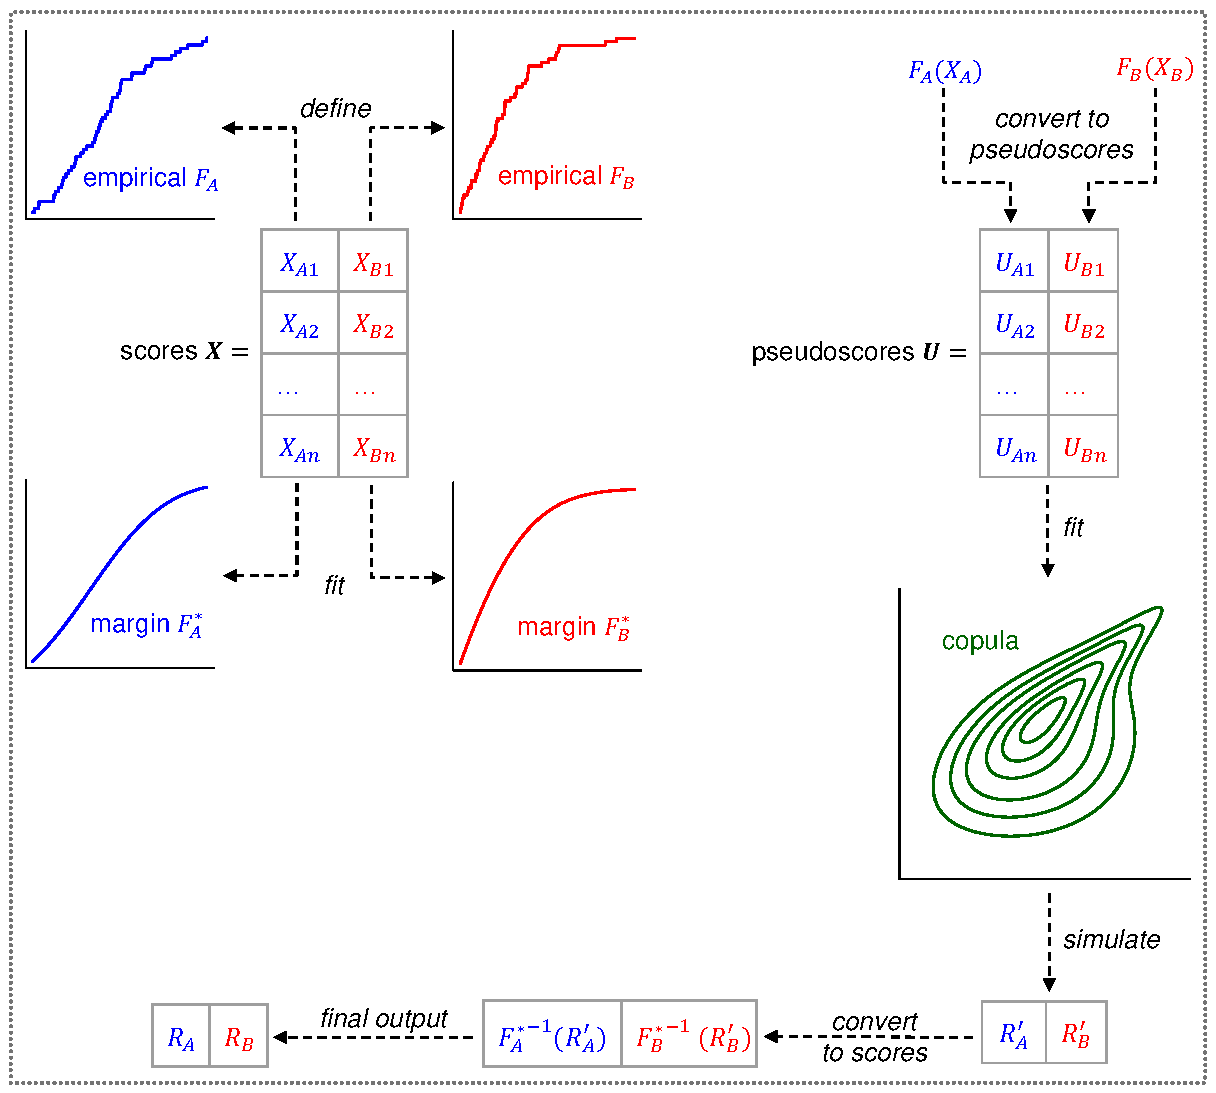
\includegraphics[width=.9\linewidth]{../diagrams/diag1_simulation}
	\caption{Schematic outline of the simulation.}	
	\label{fig:sim-diag}
\end{figure}

For any two given systems $A$ and $B$, three separate models need to be fitted, in order to be able to simulate. Two marginal models that model the marginal distribution of system $A$ and $B$ respectively, and one bi-variate copula that models the dependence between $A$ and $B$. These three models can be fitted in any order, since they are separate. 

The simulation works as follows: Let $\textbf{X}$ denote the $n \times 2$ matrix of evaluation scores of two given systems $A$ and $B$ on $n$ topics of some test collection. Let $X_A$ and $X_B$ denote the column vectors with the scores of system $A$ and $B$ respectively. To model the marginal distribution of system $A$, fit a marginal model on $X_A$. Similarly for system $B$. Let $F_A^*$ and $F_B^*$ denote the cumulative distribution function CDF of the newly fitted marginal models of system $A$ and $B$ respectively. Let $F_A$ and $F_B$ denote the empirical cumulative distribution function ECDF (Equation \ref{eq:ECDF}) of system $A$ and $B$ respectively. 

\begin{equation}\label{eq:ECDF}
	ECDF(x) = \frac{\text{number of elements in the sample} <= x}{\text{sample size}}
\end{equation}

To model the dependence between systems $A$ and $B$ a copula needs to be fitted. Copulas are actually fitted on so-called \textit{pseudo-scores}. Let $\textbf{U}$ denote the $n \times 2$ matrix of pseudo-scores, and $U_A$ and $U_B$ the column vectors with the pseudo-scores of system $A$ and $B$ respectively. Scores are converted to pseudo-scores like so: $U_A = F_A(X_A)$ and $U_B = F_B(X_B)$. A copula model is then fitted on $\textbf{U}$. 

The copula model can be used to generate \textit{paired} pseudo-observations $\{R_A^\prime, R_B^\prime\}$ of system $A$ and $B$ on a new random topic. Those two pseudo-observations are then converted to actual observations using the inverse CDF of the (previously) fitted margins, like so: $R_A = {F_A^*}^{-1}(R_A^\prime)$ and $R_B = {F_B^*}^{-1}(R_B^\prime)$.

$\{R_A, R_B\}$ is the generated pair of scores of system $A$ and $B$ on a new random topic. This procedure can be endlessly repeated to generate scores for an arbitrarily large number of new random topics.

\subsection{Marginal and Copula Families}\label{sec:families}

In order to fit a margin or a copula, several distribution families are considered, which are listed in Table \ref{tab:fams}.

%\newpage
\begin{table}[t]	
	%	\begin{minipage}{\textwidth}     	
		\centering
		\begin{tabular}{l r @{}l }
			\toprule
			\textbf{Margins} & \multirow{4}{*}{$ 
				\left.
				\begin{array}{r}
					\\
					\text{for \textit{continuous} measures}\\
					\text{(AP, nDCG@20, ERR@20)}\\
					\\
				\end{array}
				\right\lbrace$} 
			& Truncated\tablefootnote{The distributions are truncated, so that the simulated scores are within the $\left[0, 1\right]$ range, as all IR evaluation scores are.} Normal \\
			& & Truncated Normal Kernel Smoothing \\
			& & Beta \\
			& & Beta Kernel Smoothing \\
			& \multirow{2}{*}{$ 
				\left.
				\begin{array}{r}
					\text{for \textit{discrete} measures}\\
					\text{(P@10, RR)}\\
				\end{array}
				\right\lbrace$} 
			& Beta-Binomial \\
			& & Discrete Kernel Smoothing\tablefootnote{Four different variations of this distribution are considered by manipulating the smoothing parameter.} \\
			\midrule
			\midrule
			\textbf{Copulas} & & Gaussian \\
			& & Student t \\
			& & Frank \\
			& \multirow{9}{*}{$ 
				\left.
				\begin{array}{r}
					\\
					\\
					\\
					\\
					\text{including their 90, 180} \\ 
					\text{and 270 degree rotations} \\ 
					\\
					\\
					\\
				\end{array}
				\right\lbrace$} 
			& Clayton \\
			& & Gumbel \\
			& & Joe \\
			& & BB1 \\
			& & BB6 \\
			& & BB7 \\
			& & BB8 \\
			& & Tawn 1 \\
			& & Tawn 2 \\
			\bottomrule
		\end{tabular}
		\caption{List of the family distribution candidates that are considered when fitting the marginal and copula models.}
		\label{tab:fams}
		%\end{minipage}
\end{table}

For modeling the marginal distribution of a system, a simple approach that does not require model fitting would have been to use the empirical cumulative distribution function (ECDF) of the given data. However, the problem with simply using the ECDF is that the scores which were not present in the data, would never come up in the simulation. For this reason, a model is required. Furthermore, a distinction is made depending on whether or not the evaluation scores are \textit{continuous} or \textit{discrete}. This is because there are multiple effectiveness measures (i.e., AP, nDCG@20, ERR@20, P@10 and RR) and even though all of them are technically discrete, some of them have a much larger set of possible values, which makes it reasonable to treat them as continuous. 

Figure \ref{fig:fams-margin} shows a visual comparison of all candidate models for modeling the marginal distribution, in two examples. The left-hand side plot, shows all the candidate models (according to Table \ref{tab:fams}) that could be selected for modeling the marginal distribution of AP (Average Precision) scores of a system on the population of topics. Similarly, the right-hand side plot, all the candidate models that could be selected for modeling the marginal distribution of P@10 scores of another system. The original data are shown in gray color. Note that sometimes models may fail to fit, in cases where the fit is particularly bad. For example, on the right-hand side plot, two models are missing because they failed to fit. Only three models were fitted successfully, even though five models were considered (namely, the Beta-Binomial distribution plus four variations of the Discrete Kernel Smoothing distribution).

\begin{figure}[!t]
	\centering
	\begin{subfigure}{.4\textwidth}
		\centering
		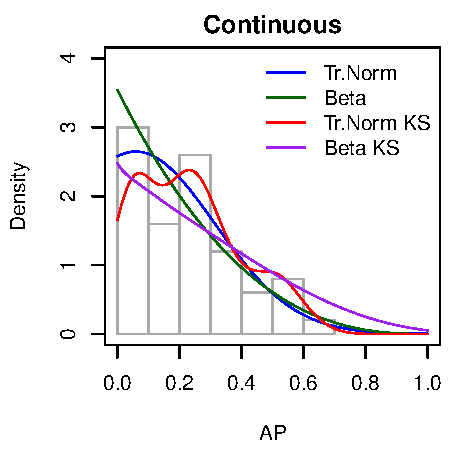
\includegraphics[width=0.95\linewidth]{margins/families_row44739_ap}
		\subcaption{System 52 from the Ad-hoc 2007 Track.}
	\end{subfigure}%
	\begin{subfigure}{.4\textwidth}
		\centering
		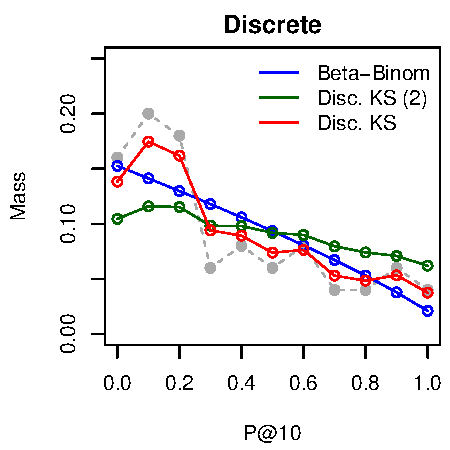
\includegraphics[width=0.95\linewidth]{margins/families_row152379_p10}
		\subcaption{System 29 from the Ad-hoc 2007 Track.}
	\end{subfigure}
	\caption{Visual comparison of the candidate marginal models. Original data in gray.}
	\label{fig:fams-margin}
\end{figure}

For modeling the dependence between the two systems, 12 copula families are considered, including some rotations. The Tawn 1 and 2 copulas are asymmetric copulas, whereas all others are symmetric. The main difference between these two categories is that when a symmetric copula is used, the distribution of the generated per-topic score differences tend to be symmetric. In contrast, asymmetric copulas may yield distributions with non-zero skewness. 

Figure \ref{fig:fams-cop} shows a visual comparison of three candidate copulas for modeling the dependence between two systems, in one example. The left-hand side plot, shows the visual difference between a symmetric (Gaussian) and an asymmetric (Tawn) copula. The right-hand side plot, shows the Independence copula for comparison, which assumes no dependency between the two systems, and the contours are perfect circles. These copulas were selected for illustration purposes, even though many more are considered (as per Table \ref{tab:fams}). The contour plots show the joint probability density function $f(x,y)$ (Equation \ref{eq:cop-density}) that is modeled with a Tawn, Gaussian and Independence copula. The reason why the joint density $f$ is plotted, as opposed to the copula density $c$, is because copula densities usually explode at some corners, which makes it difficult to visualize. A common approach is to combine the copula with standard normal margins, and plot the joint density instead, as we have done. 

\begin{figure}[t]
	\centering
	\begin{subfigure}{.4\textwidth}
		\centering
		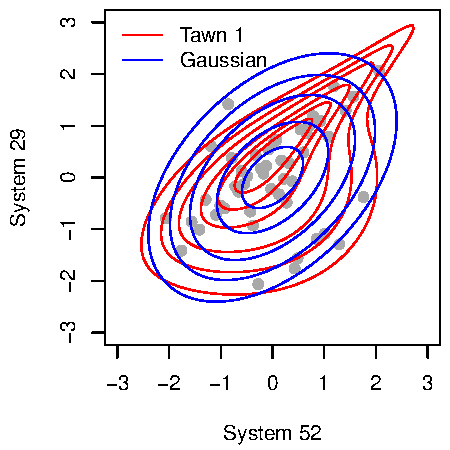
\includegraphics[width=0.95\linewidth]{copulas/families_copula_ap}
	\end{subfigure}%
	\begin{subfigure}{.4\textwidth}
		\centering
		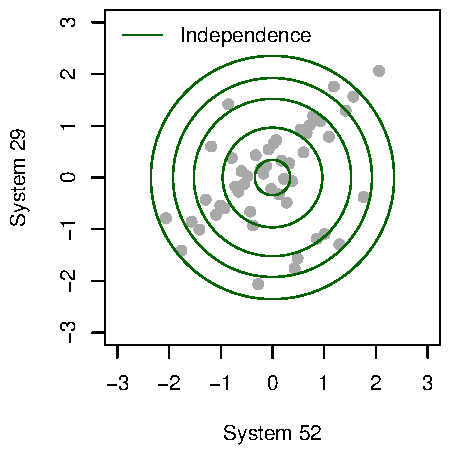
\includegraphics[width=0.95\linewidth]{copulas/families_copula_indep_ap}
	\end{subfigure}
	\caption{Visual comparison of three candidate copulas, fitted from the (paired) AP scores of systems 52 and 29 from the Ad-hoc 2007 Track. These contour plots show the joint densities, by combining the copulas with standard normal margins. Original data in gray.}
	\label{fig:fams-cop}
\end{figure}


\subsection{Model Selection Criteria}\label{criteria}

In order to fit a model, \textit{all} candidate families of Table \ref{tab:fams} are fitted first and then the best model has to be selected based on some model selection criterion. To this end, several options are available:

Log-likelihood (LL) is a basic criterion that can be used, and it is defined as the natural logarithm of the likelihood that the fitted model would have generated the observed data. Based on LL, two more criteria are defined, namely the Akaike Information Criterion (AIC) \cite{Akaike1974} and the Bayesian Information Criterion (BIC) \cite{Schwarz1978}:

\begin{equation}\label{eq:LL}
	LL = \log\left(p\left(X|\theta\right)\right)
\end{equation}

\begin{equation}\label{eq:AIC}
	AIC = -2LL + 2\kappa 
\end{equation}

\begin{equation}\label{eq:BIC}
	BIC = -2LL + \kappa\log\left(n\right)
\end{equation}

where $X$ is the observed data, $\theta$ is the vector of parameters of the model, $\kappa$ is the number of parameters of the model (or the \textit{effective degrees of freedom} in case the model is non-parametric) and $n$ is the sample size (the number of topics).

For the case of LL, the model with the highest value is selected. The opposite is true for the case of AIC and BIC, where the model with the lowest value is selected. All three criteria are probabilistic measures that estimate a model's performance on the same data that was used to fit that model. This means that their computation does not require a hold-out set. The main difference between the three criteria is that AIC and BIC penalize complex models, and therefore favor simple models. LL can be problematic because it might favor models that are overly complex, and those models are often the result of overfitting. BIC penalizes models harsher than AIC, if $n \geq 8$. 

\section{Related Work}

One application of the aforementioned simulation is that it can be used as a tool to study which statistical significance test is optimal for IR evaluation data. Statistical significance tests are used to assess if an observed difference in mean system performance is real, as opposed to an error due to the sampling of topics. This is because systems are evaluated on a mere sample of topics rather than the entire population of topics, and for this reason there is some random noise associated with evaluation results. There are various statistical significance tests, for example the Student’s t-test, Wilcoxon test, Sign test, Bootstrap test and Permutation test. Every test relies on certain assumptions that are typically not satisfied by IR evaluation data. For example, the t-test assumes that the data are normally distributed, which is not true. 

Most commonly, researchers are interested in comparing only two systems; an experimental system against a baseline system. To achieve this, the two systems are typically evaluated on the same test collection and as a consequence on the same set of topics. For this reason, the evaluation results are in the form of \textit{paired} per-topic scores. After the results are obtained, if it is observed that the experimental system outperformed the baseline system, then a so-called \textit{paired} statistical significance test is run, to determine if this observed difference in mean system performance is statistically significant or not. In other, rarer cases where a researcher wants to compare $N$ systems as opposed to only two, ANOVA models are used instead.

The simulation approach we discussed in Section \ref{sec:sim-description}, was applied in \cite{Urbano2019}, in order to study how well statistical significance tests really behave on IR evaluation data. The authors studied an extensive range of different factors, while focusing on the specific (but popular) case of \textit{paired} tests. In such tests, only two systems (as opposed to $n$ systems) are compared. In order to compare the various statistical significance tests, the main requirement is to estimate their Type I and Type II error rates. One way of accomplishing this, is by employing stochastic simulation.

In order to study Type I error rates, the following process is repeated. For a target effectiveness measure and topic set size, two systems $B$ and $E$ are randomly selected from the same collection. Then, two marginal models ($F_B$ and $F_E$) and a copula are fitted on the data. The model selection is done using AIC. For computing Type I error rates, the data are generated under the null hypothesis $H_0: μ_E = μ_B$. This is achieved by assigning $F_E \leftarrow F_B$ after the margins have been fitted. After the simulation, the significance tests are then run on the newly generated data. Any statistically significant result counts as a Type I error, due to the fact that the data were generated under the null hypothesis.

In order to study Type II error rates, the process is similar. However, this time the data need to be generated under the alternative hypothesis $H_A: μ_E = μ_B + \delta$. This requirement is achieved in two steps. Firstly, system $B$ is selected from the bottom 75\% performing systems, and system $E$ is selected at random from the set of 10 systems whose mean is closest to the target $μ_B + \delta$. Secondly, after the margins have been fitted, a small transformation is performed on $F_E$, such that the condition $μ_E = μ_B + \delta$ holds true. After the simulation, the significance tests are then run on the newly generated data. Any result that does not come up as statistically significant, counts as a Type II error, due to the fact that the data were generated under a false null hypothesis.

Their findings suggest that the t-test and Permutation tests are the most optimal, whereas the Wilcoxon, Sign and Bootstrap-Shift test are the least optimal. The authors' top recommendation is the t-test.

Beyond the line of work of Urbano et al., there is another recent line of work by Parapar et al. \cite{Parapar2020, Parapar2021}, that also relies on simulation. In \cite{Parapar2020}, for every system-topic pair, a model is built that models the \textit{retrieval score} distribution (SD) \cite{Manmatha2001}. The term retrieval score refers to the score that the system itself gives to each document, in order to rank the documents from best to worst, during the retrieval process. The model used is a mixture of two log-normal distributions: one for relevant and the other for non-relevant documents. 

In order to study Type I error rates, the following process is repeated. A system is randomly selected, and all (50) of its mixture models are used to generate two outputs each. The outputs are \textit{synthetic} lists of 1000 retrieval scores and corresponding relevance values, sorted from best to worst retrieval score. For each output, Average Precision (AP) is computed. The statistical significance tests are then run on the two resulting sequences of 50 AP scores. Any statistically significant result is a Type I error, because the data were generated under the null hypothesis, since they come from the same system. 

In order to study Type II error rates, the approach is similar. The difference is that instead of generating two outputs per mixture model, one output is generated instead. Then, the parameter of the model is altered, and the second output is generated. The model is altered by increasing the true mean of the (log-normal) distribution for the relevant documents. This way, the data are generated under some alternative hypothesis.

In a more recent paper \cite{Parapar2021}, the work done in \cite{Parapar2020} was improved by the same authors. The approaches used in the two papers are very similar. The main difference is in the simulation methodology. Given a system-topic pair, a model is build that captures the relationship between document ranks and relevance. More specifically, for a system-topic pair, a logistic regression model is fitted, where the target variable is relevance, and the only predictor is the position of the document in the ranking. In order to simulate a new ranking, for every position $p$ in ${\{1, 2, ..., 1000\}}$, the value $h_\theta(p)$ is obtained (from the fitted Logistic model $h_\theta$). The relevance value of the new ranking at position $p$ is determined by drawing a sample from a Bernoulli distribution with parameter $h_\theta(p)$. This way a sequence of 0s and 1s is generated, which is sufficient for computing Average Precision. Studying Type I and Type II errors is done in the same manner. One difference is in regard to studying Type II errors, where the parameters $\theta_0$ and $\theta_1$ of the logistic regression model are manipulated in order to simulate under some alternative hypothesis. 

Surprisingly, the authors reach opposite conclusions. The biggest disagreement in terms of recommendations is regarding the Wilcoxon test and the t-test, where the conclusions are opposite. 

Parapar et al., in \cite{Parapar2021}, provide some empirical results regarding the quality of the simulation used in that paper. This was done by computing the average correlation between original ranking and simulated rankings of the system-topic pairs. Their results showed that the simulated rankings only differ slightly compared to the original, and it is argued that this is a good sign of quality, because the generated rankings should represent the original. However, this is arguably not a very comprehensive analysis, because according to this comparison, adding a small noise to the rankings would be considered a simulation of high quality.

Thus far, no empirical evidence have been produced regarding the quality of the simulation used in the line of work of Urbano et al., which is the main objective of this thesis.
